\section{Gewöhnliche Differentialgleichungen}

%%%%%%%%%%%%%%%%%%%%%%%%%%%%%%%%%%%%%%%%%%%%%%%%%%%%%%%%%%%%
%%%%%%%%%%%%%%%%%%%%%%%%%%%%%%%%%%%%%%%%%%%%%%%%%%%%%%%%%%%%
\subsection{Modellierung mit Differentialgleichungen}

\begin{frame}{Ausgangsfragestellung}
  \begin{columns}
    \begin{column}{.6\textwidth}
      \begin{itemize}
      \item<+-> Anzucht von Hefe
      \item<+-> Fermenter
      \item<+-> Fragen:
        \begin{itemize}
        \item<+-> Kann ich für einen beliebigen Zeitpunkt die Anzahl
          an Hefezellen vorhersagen?
        \item<+-> Wie lange muss ich warten, bis ich die gewünschte Ausbeute habe?
        \end{itemize}
      \end{itemize}
    \end{column}
    \begin{column}{.38\textwidth}
      \begin{center}
        \only<2->{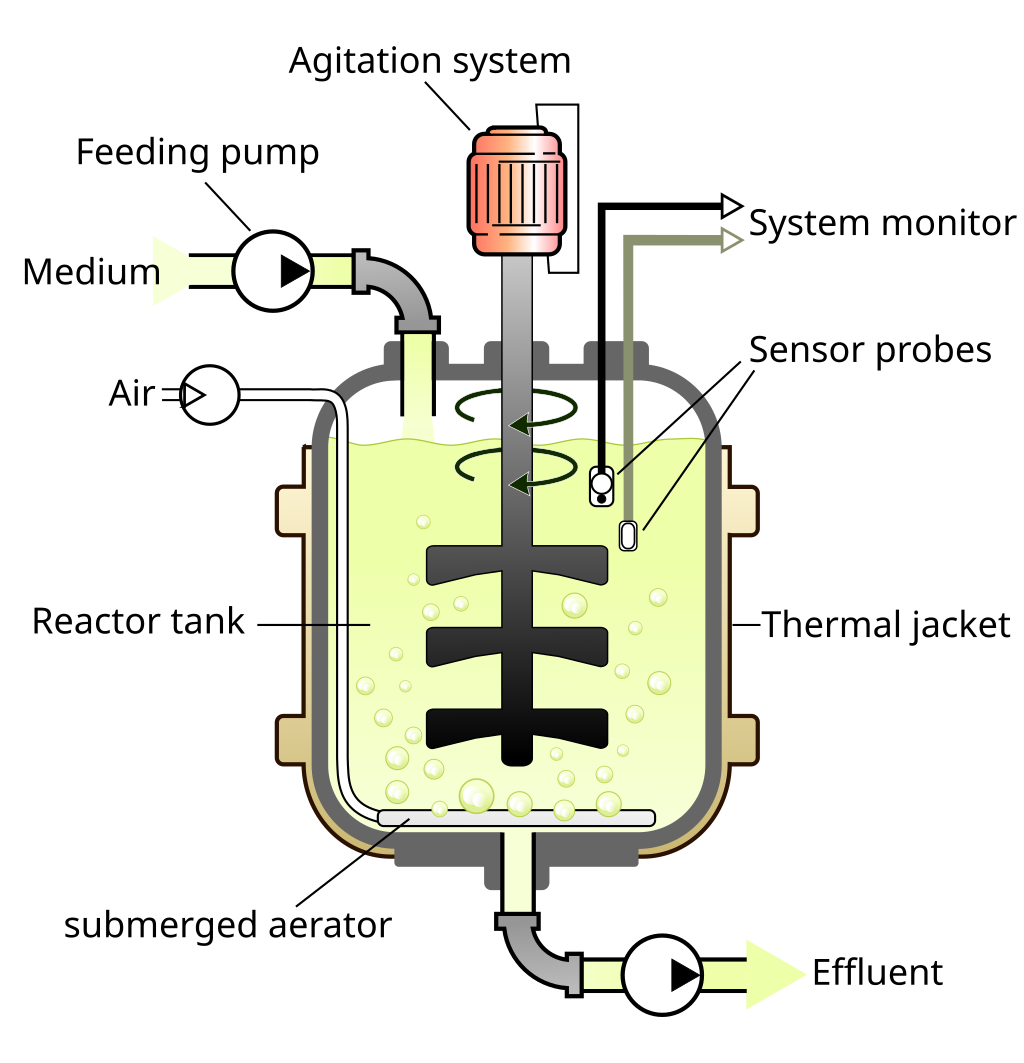
\includegraphics[width=.9\textwidth]{fig/Bioreactor}

          \tiny © Yassine Mrabet, Wikipedia
        }
      \end{center}
    \end{column}
  \end{columns}
\end{frame}

\begin{frame}
  \begin{exampleblock}{Frage}
    Welche Informationen benötigen Sie, um diese Aufgabe zu lösen?
  \end{exampleblock}
\end{frame}

\begin{frame}
  \begin{block}{Verdopplungsrate}
    Under optimal conditions, yeast cells can double their population every 100 minutes.

    \begin{flushright}
      \tiny Wikipedia: Saccaromyces cerevisiæ
    \end{flushright}
  \end{block}

  \pause
  \vspace{5mm}
  
  \begin{tikzpicture}[scale=.9]\footnotesize
    \draw [->] (0,0) -- (12.5,0);
    \draw (0,.1)  -- (0,-.1) node[below] {8:00};
    \draw (2,.1) -- (2,-.1) node[below] {9:40};
    \draw (4,.1) -- (4,-.1) node[below] {11:20};
    \draw (6,.1) -- (6,-.1) node[below] {13:00};
    \draw (8,.1) -- (8,-.1) node[below] {14:40};
    \draw (10,.1) -- (10,-.1) node[below] {16:20};
    \draw (12,.1) -- (12,-.1) node[below] {18:00};
    \only<2>{
      \path (1,.3) node {2x};
      \path (3,.3) node {2x};
      \path (5,.3) node {2x};
      \path (7,.3) node {2x};
      \path (9,.3) node {2x};
      \path (11,.3) node {2x};
    }
    \only<3->{
      \path (0.,.1) node[above,red!60!black]{1000};
      \path (2.,.1) node[above,red!60!black]{2000};
      \path (4.,.1) node[above,red!60!black]{4000};
      \path (6.,.1) node[above,red!60!black]{8000};
      \path (8.,.1) node[above,red!60!black]{16000};
      \path (10.,.1) node[above,red!60!black]{32000};
      \path (12.,.1) node[above,red!60!black]{64000};
    }
    \only<4>{
      \draw[green!45!black] (7,.1) -- (7,-.1) node[below,green!45!black] {13:50};
    }
  \end{tikzpicture}

  \pause
  \vspace{5mm}

  \begin{block}{Anfangspopulation}
    Beispiel: Die Population um 8:00 beträgt 1000 Zellen
  \end{block}
  \pause
  \begin{exampleblock}{Frage}
    Wieviele Zellen haben wir um 13:50?
  \end{exampleblock}
\end{frame}

\begin{frame}{Mathematisch etwas allgemeiner und präziser...}
  \begin{itemize}
  \item Anzahlvariable $N$
  \item Zeitvariable $t$ in Minuten, Startzeit $t_0=8:00$, ``Messzeit'' $T=18:00$
  \item Zeitintervalle $I_k = [t_{k},t_{k+1}]$ der Länge $\Delta t = 100 \text{min}$
    
    \vspace{5mm}
    \hspace*{-1ex}
  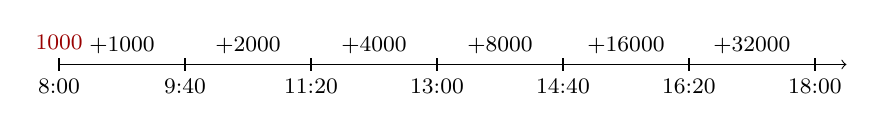
\begin{tikzpicture}[scale=.8]\footnotesize
    \draw [->] (0,0) -- (12.5,0);
    \draw (0,.1)  -- (0,-.1) node[below] {8:00};
    \draw (2,.1) -- (2,-.1) node[below] {9:40};
    \draw (4,.1) -- (4,-.1) node[below] {11:20};
    \draw (6,.1) -- (6,-.1) node[below] {13:00};
    \draw (8,.1) -- (8,-.1) node[below] {14:40};
    \draw (10,.1) -- (10,-.1) node[below] {16:20};
    \draw (12,.1) -- (12,-.1) node[below] {18:00};
      \path (0.,.1) node[above,red!60!black]{1000};
      \path (1,.3) node {+1000};
      \path (3,.3) node {+2000};
      \path (5,.3) node {+4000};
      \path (7,.3) node {+8000};
      \path (9,.3) node {+16000};
      \path (11,.3) node {+32000};
    \end{tikzpicture}

    \vspace{5mm}
    
  \item Sei $d_k$ der Zuwachs im Intervall $I_k$
    \begin{gather*}
      N(t_{k+1}) = N(t_k) + d_k,
      \qquad N(T) = N(t_0) + \sum_{k=0}^{n-1} d_k.
    \end{gather*}
  \end{itemize}
  \pause
  \begin{exampleblock}{Frage}
    Im Beispiel ist $d_k=N(t_k)$. Wie ändert sich $d_k$ qualitativ, wenn wir die Intervalle halbieren?
  \end{exampleblock}
\end{frame}

%%%%%%%%%%%%%%%%%%%%%%%%%%%%%%%%%%%%%%%%%%%%%%%%%%%%%%%%%%%%
\begin{frame}{Halbierung der Intervalle}
  \begin{tikzpicture}[scale=3]\footnotesize
    \draw [thick,->] (6.,0) -- (8.5,0);
    \draw (6,.1) node[above] {8000} -- (6,-.1) node[below] {13:00};
    \draw (8,.1) node[above] {16000} -- (8,-.1) node[below] {14:40};
    \path (7,.3) node {+8000};

    \draw [thick,->] (6.,-.7) -- (8.5,-.7);
    \draw (6,-.6) -- (6,-.8) node[below] {13:00};
    \draw (8,-.6) -- (8,-.8) node[below] {14:40};
    \draw (7,-.6) node[above] {\textcolor{red!60!black}{\only<1>{???}\only<3->{11314}}} -- (7,-.8) node[below] {13:50};
    \path (6.5,-.5) node {\textcolor{red!60!black}{\only<1>{+???}\only<3->{3314}}};
    \path (7.5,-.5) node {\textcolor{red!60!black}{\only<1>{+???}\only<3->{4686}}};
  \end{tikzpicture}

  \only<1>{\begin{Denkpause}
      Welche Werte sollten für die Fragezeichen stehen?
    \end{Denkpause}}
  \pause
  \begin{itemize}
  \item Die Summe sollte 8000 ergeben
  \item Der Quotient aus Summand und linkem Wert sollte gleich sein
  \end{itemize}
\end{frame}


\begin{frame}{Lösung von der Intervallänge}
  \begin{itemize}
  \item Es gilt eine Beziehung wie
    $d_k \approx f(t_k)\Delta t$.
  \item Die Funktion $f$ gibt an, wieviele Hefezellen im Zeitintervall
    der Länge $\Delta t$ entstehen
  \item Sie hängt von der aktuellen Anzahl ab
  \item Dann können wir für eine beliebige Folge von $n$ Intervallen
    schreiben
    \begin{gather*}
      N(t_n) = N(t_0) + \sum_{k=0}^{n-1} f(t_k) (\Delta t)_k
    \end{gather*}
    \only<1>{
      \begin{Denkpause}
        Wo haben wir eine solche Modellierung schon gesehen?
      \end{Denkpause}
}
    \pause
    \item Wenn wir die Intervalllänge gegen null gehen lassen, bekommen wir ein Integral
  \end{itemize}
\end{frame}

\begin{frame}
  \begin{itemize}
  \item<+-> Für individuelle Hefezellen ist $\Delta t \to 0$ unsinnig,
    weil sich ab einem Punkt sehr wahrscheinlich keine einzige Zelle
    in einem Intervall vermehrt.
    \item<+-> Wir ersetzen daher die diskrete Anzahl $N(t)$ durch eine
    kontinuierliche Größe $x(t)$ z. B. mit der Einheit Gramm anstelle
    von Stück.
  \end{itemize}
  \begin{block}<+->{Kontinuumshypothese} Wir nehmen an, dass der
    Übergang von einer diskreten zu einer kontinuierlichen Größe keine
    großen Fehler verursacht.
    \begin{itemize}
    \item Die Werte $x \sim N$ und $x\sim N+1$ unterscheiden sich kaum
    \item Statistische Fluktuationen des Zuwachses $d_k$ haben keinen
      merkbaren Einfluss
    \end{itemize}
  \end{block}

  \begin{itemize}
  \item<+-> Hefe: 1 Gramm entspricht $10^9$ Zellen
  \item<+-> Verdopplung entspricht $10^9$ Zellteilungen in 2 Stunden
  \end{itemize}
\end{frame}

\begin{frame}{Integraldarstellung}
  Ersetzen wir $N(t)$ durch $x(t)$ und lassen die Summen konvergieren, so erhalten wir die \textbf{Volterrasche Integralgleichung}
    \begin{gather*}
      x(T) = x(t_0) + \int_{t_0}^T f(t) \dt.      
    \end{gather*}
  \begin{block}{Instantane Reproduktionsrate $R$}
    Für die Funktion unter dem Integral setzen wir
    \begin{gather*}
      f(t) = R x(t).
    \end{gather*}
    Hier repräsentiert $R$ eine Reproduktionsrate für ein unendlich kleines Zeitintervall $dt$.
    %, also
    % \begin{gather*}
    %   R = \lim_{h\to 0} \tfrac{x(t+h)-x(t)}{h}.
    % \end{gather*}
  \end{block}
\end{frame}

\begin{frame}
  Wir erhalten die Darstellung der Funktion $x(t)$ als
  \begin{block}{Volterrasche Integralgleichung}
    \begin{gather*}
      x(t) = x(t_0) + \int_{t_0}^t R x(s) \ds.      
    \end{gather*}    
  \end{block}

  Differenzieren wir auf beiden Seiten ergibt die Darstellung als
  \begin{block}{Differentialgleichung}
    \begin{gather*}
          x'(t) = R x(t)
    \end{gather*}
  \end{block}
\end{frame}

\begin{frame}{Lösungen}
  Aus der Schule ist die Exponentialfunktion bekannt. Es gilt:
  \begin{gather*}
    \tfrac d{dt} e^{Rt} = R e^{Rt}.
  \end{gather*}
  Dies gilt aber auch für alle Funktionen $x(t) = c \,e^{Rt}$ mit einer Konstanten $c$.

  \begin{block}{Anfangswertaufgabe}
    Die Lösungsgesamtheit der Differentialgleichung $x' = Rx$ besteht
    aus allen Funktionen der Form $c\,e^{Rt}$.

    \vspace{1ex}

    Die tatsächliche Lösung erhält man, indem man die Konstante an den Anfangswert $x_0$ angleicht:
    \begin{gather*}
      x_0 = x(t_0) = c e^{Rt_0} \qquad \Rightarrow \qquad c = \frac{x_0}{e^{R t_0}}
    \end{gather*}
  \end{block}
\end{frame}

\begin{frame}{Berechnung von $R$}
  Wenn $\Delta t$ die Zeit zur Verdopplung ist, wie groß ist $R$?
  \begin{itemize}
  \item Wenn $x(0) = x_0$, so gilt $x(T)=2x_0$ nach der Verdopplungszeit
    $T=100 \,\text{min}$
  \item Wir können nun rechnen
    \begin{gather*}
      2 x_0 = x_0 e^{RT}
      \quad\Leftrightarrow\quad
      2 = e^{RT}
      \quad\Leftrightarrow\quad
      \ln 2 = RT
    \end{gather*}
  \item Wir erhalten den Wert
    \begin{gather*}
      R=\frac{\ln 2}{100} \,\text{min}^{-1}  \approx 0.00693 \,\text{min}^{-1}
    \end{gather*}
  \end{itemize}
\end{frame}

\begin{frame}{Einheiten}
  \begin{minipage}{.9\textwidth}
  \begin{itemize}
  \item Wir setzen Einheiten für $t$ und $x$, zum Beispiel
    \begin{gather*}
      t[\text{min}],\qquad x[\text{g}].
    \end{gather*}
  \item Dann hat $x'$ die Einheit $\nicefrac{\text{g}}{\text{min}}$
  \item Wegen
    \begin{gather*}
      R = \frac{x'}{x} \qquad\text{ist die Einheit von $R$ dann}\quad R[\nicefrac1{\text{min}}]
    \end{gather*}
  \end{itemize}    
  \end{minipage}
  \pause
  \begin{block}{Dimensionslose Formulierung}
    Indem man formal durch die Einheiten teilt, werden die Gleichungen
    dimensionslos.

    \vspace{1ex}

    Man kann auch durch charakteristische Größen teilen, um gezielt
    mathematisch einfache Darstellungen zu erhalten.
  \end{block}
\end{frame}

\begin{frame}
  \frametitle<presentation>{Änderung der Einheiten}
  Wir wollen im obigen Beispiel die Zeiteinheit auf Stunden wechseln
  \begin{itemize}
  \item Aus der Beziehung $\ln 2 = RT$ folgt, dass das Produkt der
    Einheiten von $R$ und $T$ einheitenlos sein muss.
  \item Für die Einheiten $T[\text{min}]$ und $R[\text{min}^{-1}]$
    haben wir den Wert von $R$ berechnet.
  \item Wollen wir die Zeiteinheit auf Stunden umrechnen, so müssen
    wir auch den Wert von $R$ mit 60 multiplizieren, also
    \begin{gather*}
      R = \ln 2\frac35\,\text{h}^{-1} \approx 0.416
    \end{gather*}
  \end{itemize}
\end{frame}

\begin{frame}{Charakteristische Zeit}
  \begin{itemize}
  \item Die Verdopplungszeit ist ein Beispiel für eine Charakteristische Zeit
  \item Üblicher: die Zeit, in der die Lösung um den Faktor $e$ zunimmt.
  \item Sei $T$ diese Zeit in irgendeiner Einheit,
    \begin{itemize}
    \item die Zeit mit derselben Einheit $\hat t$,
    \item die dimensionslose Zeit $t= \hat t/T$.
    \end{itemize}
    \pause
  \item Dann gilt für $x(t)$
    \begin{gather*}
      x(1) = x_0 e^{1R} = x_0 e^{R}
    \end{gather*}
    \pause
  \item In dieser Darstellung ist also $R=1$
  \item $R$ ist hier wie $t$ dimensionslos
  \end{itemize}
\end{frame}

%%%%%%%%%%%%%%%%%%%%%%%%%%%%%%%%%%%%%%%%%%%%%%%%%%%%%%%%%%%%%%%%%%%%%%

\begin{frame}
  \only<1>{%
    \begin{Denkpause}
      Was passiert für $t\to\infty$?
    \end{Denkpause}
    
    \begin{Denkpause}
      Was passiert für $t\to\infty$ falls $R<0$?    
    \end{Denkpause}
  }
  \pause
  \begin{itemize}
  \item<+-> Für $R>0$ nimmt die Hefe-Population unbegrenzt und exponentiell zu
    \begin{itemize}
    \item Das ist nicht sehr realistisch
    \end{itemize}
  \item<+-> Für $R<0$ stirbt die Hefe exponentiell aus
  \end{itemize}
\end{frame}

\begin{frame}
  \begin{Denkpause}
    Was erwarten Sie im Fermenter, wenn Sie im Prozess keine Nahrung
    zuführen? Betrachten Sie vor allem den Fall $t\to\infty$.
  \end{Denkpause}

  \begin{Denkpause}
    Was erwarten Sie im Fermenter, wenn Sie im Prozess mit konstanter
    Rate Nahrung zuführen? Betrachten Sie vor allem den Fall
    $t\to\infty$.
  \end{Denkpause}
\end{frame}

\begin{frame}{Modellierung}
  \begin{itemize}
  \item Bisher hatten wir $R$ bei optimalen Bedingungen
    \begin{itemize}
    \item Nahrungsmenge $F_{\text{opt}}$
    \end{itemize}
  \item Bei Nahrungszufuhr $F_{\text{opt}}$ ist der Anteil an verfügbarer Nahrung $1-Vx$
    \begin{itemize}
    \item $V$ der spezifische Verbrauch der Hefe
    \end{itemize}
  \item Jetzt setzen wir unter Vereinfachung für die Reproduktionsrate
    \begin{gather*}
      r = R \frac{F}{F_{\text{opt}}} = R (1-Vx)
    \end{gather*}
  \item Wir erhalten die ``logistische Differentialgleichung''
    \begin{gather*}
      x' = rx = R (1-Vx) x.
    \end{gather*}
  \end{itemize}
\end{frame}

\begin{frame}
  \begin{block}{Lösungen}
    \begin{gather*}
      x_c(t) = \frac{e^{Rt}}{V e^{Rt}+c}
    \end{gather*}
  \end{block}
  \only<1>{
    \begin{Denkpause}
      Glauben Sie mir diese Lösung?
    \end{Denkpause}
  }
  \pause
  \begin{itemize}
  \item Für $t\to\infty$ sind diese Lösungen beschränkt:
    \begin{itemize}
    \item Für $R>0$ konvergiert $x_c(t) \to 1/V$
    \item Für $R<0$ konvergiert $x_c(t) \to 0$
    \end{itemize}
  \end{itemize}
\end{frame}


%%%%%%%%%%%%%%%%%%%%%%%%%%%%%%%%%%%%%%%%%%%%%%%%%%%%%%%%%%%%%%%%%%%%%%
\begin{Abschluss}
\item Wie kann man das Zeitverhalten von Wachstumsprozessen modellieren?
\item Was ist die Kontinuumshypothese?
\item Wie hängen Volterrasche Integralgleichung und Differentialgleichung zusammen?
\item Was ist exponentielles Wachstum?
\item Wie modelliert man Populationsentwicklung bei beschränkten Ressourcen?
\item Wie überprüft man die Lösung einer Differentialgleichung?
\end{Abschluss}
  
%%%%%%%%%%%%%%%%%%%%%%%%%%%%%%%%%%%%%%%%%%%%%%%%%%%%%%%%%%%%%%%%%%%%%% 
%%%%%%%%%%%%%%%%%%%%%%%%%%%%%%%%%%%%%%%%%%%%%%%%%%%%%%%%%%%%%%%%%%%%%%
\subsection{Grundbegriffe}

%%%%%%%%%%%%%%%%%%%%%%%%%%%%%%%%%%%%%%%%%%%%%%%%%%%%%%%%%%%%
\begin{frame}
  \begin{block}{Differentialgleichung}
    Eine Differentialgleichung ist eine Gleichung, die eine Funktion
    und/oder ihre Ableitungen in Beziehung setzt.
  \end{block}
  \begin{columns}
    \begin{column}[t]{.49\textwidth}
      \begin{block}{Gewöhnliche DGl.}
        Es kommen nur Ableitungen bzgl. einer Variablen vor. Beispiel:
        \begin{gather*}
          x^{(3)}(t) + \sin(t) x'(t) = x^2(t) +t^2
        \end{gather*}
      \end{block}
    \end{column}
    \begin{column}[t]{.49\textwidth}
      \begin{block}{Partielle DGl.}
        Es kommen partielle Ableitungen nach mehreren Variablen vor.
        Beispiel:
        \begin{gather*}
          \partial_t u(t,x) - \partial_{xx} u(t,x) = \sin(x)
        \end{gather*}
      [Nicht in dieser Vorlesung]
      \end{block}
    \end{column}
  \end{columns}
  \pause
  \begin{block}{Ordnung einer Differentialgleichung}
    Die Ordnung einer DGl. ist der Grad der höchsten Ableitung, die in
    der Gleichung vorkommt.
  \end{block}
\end{frame}

%%%%%%%%%%%%%%%%%%%%%%%%%%%%%%%%%%%%%%%%%%%%%%%%%%%%%%%%%%%%
\begin{frame}{Systeme gewöhnlicher Differentialgleichungen}
  \begin{itemize}
  \item Ein System gewöhnlicher
    Differentialgleichungen erster Ordnung hat die Form
    \begin{align*}
      x_1'(t) &= f_1\bigl(t,x_1(t),\dots,x_n(t) \bigr)\\
      x_2'(t) &= f_2\bigl(t,x_1(t),\dots,x_n(t) \bigr)\\
      \vdots\\
      x_n'(t) &= f_n\bigl(t,x_1(t),\dots,x_n(t) \bigr)
    \end{align*}
  \item  $n$ ist die Dimension des Systems
  \item Einfacher in Vektorschreibweise
    \begin{gather*}
      \vx'(t) = \vf\bigl(t,\vx(t)\bigr)
    \end{gather*}
  \item Die Funktion $\vx$ beschreibt einen Weg in $\R^n$, auch \textbf{Trajektorie} genannt
  \end{itemize}
\end{frame}

%%%%%%%%%%%%%%%%%%%%%%%%%%%%%%%%%%%%%%%%%%%%%%%%%%%%%%%%%%%%
\begin{frame}
  \begin{itemize}
  \item   Jede Differentialgleichung $n$-ter Ordnung
    \begin{gather*}
      F\bigl(t,x^{(n)},x^{(n-1)},\dots,x',x\bigr) = 0
    \end{gather*}
    lässt sich als System erster Ordnung der Dimension
    $n$ schreiben! Mit $x_1=x$:
    \begin{align*}
      x_1' &= x_2\\
      \vdots\\
      x_{n-1}' &= x_n\\
      F\bigl(t,x_n', x_n,\dots,x_1\bigr)&=0 
    \end{align*}
  \item Durch Auflösen nach $x_n'$ ist die Form
    \begin{gather*}
      \vx' = \vf\bigl(t,\vx\bigr)    
    \end{gather*}
    damit der allgemeine Fall.
    \begin{itemize}
    \item Die Argumente \glqq$t$\grqq{} lassen wir oft weg
    \end{itemize}
  \end{itemize}
\end{frame}

%%%%%%%%%%%%%%%%%%%%%%%%%%%%%%%%%%%%%%%%%%%%%%%%%%%%%%%%%%%%
\begin{frame}
  \begin{block}{Autonome Differentialgleichungen}
    Eine Differentialgleichung heißt autonom, wenn keiner der Terme
    eine explizite Abhängigkeit von der Zeit hat.
  \end{block}
  \begin{columns}
    \begin{column}[t]{.49\textwidth}
      \begin{block}{Autonom}
        \begin{gather*}
          \vx' = \vf(\vx)
        \end{gather*}
      \end{block}
    \end{column}
    \begin{column}[t]{.49\textwidth}
      \begin{block}{Nicht autonom}
        \begin{gather*}
          \vx' = \vf(t,\vx)
        \end{gather*}
      \end{block}
    \end{column}
  \end{columns}
  \pause
  \begin{Denkpause}
    Welche Prozesse führen zu autonomen DGln., welche zu nicht autonomen?
  \end{Denkpause}
\end{frame}

%%%%%%%%%%%%%%%%%%%%%%%%%%%%%%%%%%%%%%%%%%%%%%%%%%%%%%%%%%%%
\begin{frame}
  \frametitle<presentation>{Modellierung mit autonomen Dgln.}
  \begin{itemize}
  \item Annahme: Zeitinvarianz,  konstante äußere Bedingungen
    \begin{itemize}
    \item Naturgesetze
    \item Temperatur
    \item Nährstoffzufuhr
    \item pH-Wert
    \item etc.
    \end{itemize}
  \item Beispiele: Reaktionsnetzwerke, metabolische Dynamik
  \item Bei autonomen DGln. ist der Startzeitpunkt frei
  verschiebbar, wir wählen oft $t_0 = 0$.
  \end{itemize}
\end{frame}


%%%%%%%%%%%%%%%%%%%%%%%%%%%%%%%%%%%%%%%%%%%%%%%%%%%%%%%%%%%%
\begin{Abschluss}
\item Was ist die Ordnung einer Differentialgleichung?
\item Was sind Systeme von Dgln.?
\item Welche Darstellung genügt?
\item Wie zeichnen sich autonome Dgln. aus?
\end{Abschluss}


%%%%%%%%%%%%%%%%%%%%%%%%%%%%%%%%%%%%%%%%%%%%%%%%%%%%%%%%%%%%
%%%%%%%%%%%%%%%%%%%%%%%%%%%%%%%%%%%%%%%%%%%%%%%%%%%%%%%%%%%%
\subsection{Richtungsfelder und Fixpunkte}

\begin{frame}{Richtungsfelder}
  \begin{itemize}
  \item Die Lösung $x(t)$ einer Differentialgleichung kann als Weg
    $(t,x(t))$ dargestellt werden
  \item Der Geschwindigkeitsvektor beschreibt die Änderung
    in der Zeit:
    \begin{gather*}
      \begin{pmatrix}
        t'\\x'(t)
      \end{pmatrix}
      =
      \begin{pmatrix}
        1\\f(t,x)
      \end{pmatrix}
    \end{gather*}
  \item Zu jedem Punkt in der $(t,x)$-Ebene ist ein solcher Vektor
    durch die Differentialgleichung gegeben
  \item Dieses \textbf{Richtungsfeld} erlaubt die graphische
    Rekonstruktion der Lösung $x(t)$
  \end{itemize}
\end{frame}

\begin{frame}{Richtungsfeld der logistischen Dgl.}
  \begin{columns}
    \begin{column}[t]{.2\textwidth}
    \begin{gather*}
      x'= (1-x) x
    \end{gather*}
    \begin{exampleblock}{Frage}
      Verhalten für $t\to\infty$
    \end{exampleblock}
    \end{column}
    \begin{column}[t]{.78\textwidth}
      \mbox{}
      
      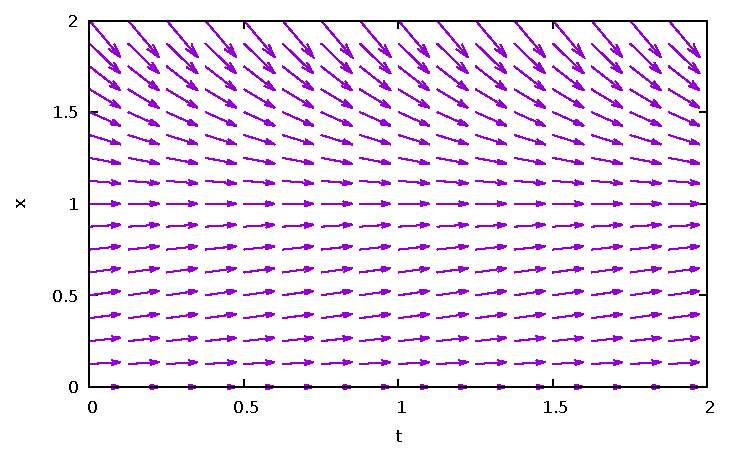
\includegraphics[width=\textwidth]{gnuplot/logistic.pdf}
    \end{column}
  \end{columns}
\end{frame}

\begin{frame}
  \frametitle<presentation>{Negative Startwerte}
  \begin{columns}
    \begin{column}[t]{.2\textwidth}
    \begin{gather*}
      x'= (1-x) x
    \end{gather*}      
    \end{column}
    \begin{column}[t]{.78\textwidth}
      \mbox{}
      
      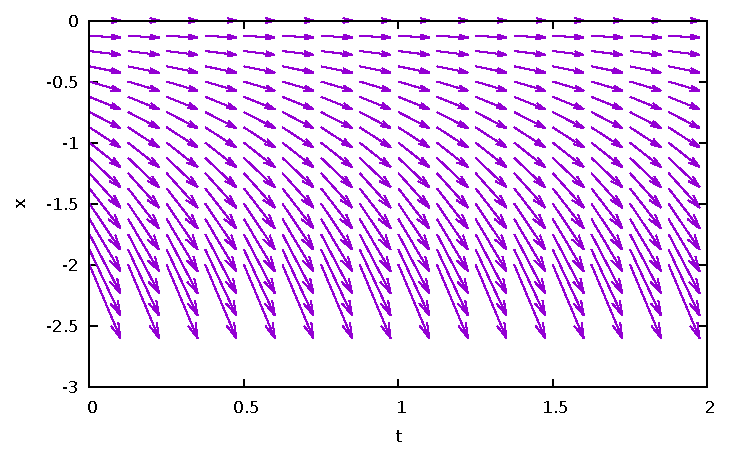
\includegraphics[width=\textwidth]{gnuplot/logisticm.pdf}
    \end{column}
  \end{columns}
\end{frame}

%%%%%%%%%%%%%%%%%%%%%%%%%%%%%%%%%%%%%%%%%%%%%%%%%%%%%%%%%%%%
\begin{frame}{Weiteres Beispiel Richtungsfeld}
  \includegraphics[width=.8\textwidth]{gnuplot/sinelog.pdf}
  \only<1>{\begin{Denkpause}
      Was unterscheidet dieses Richtungsfeld vom vorherigen?
      
      Was für einen anderen Gleichungtyp zeigt es?
    \end{Denkpause}}
  \pause
  \begin{itemize}
  \item Keine autonome Gleichung, Richtung hängt von $t$ ab
  \end{itemize}
\end{frame}

\begin{frame}{Fixpunkte}
  \begin{itemize}
  \item Für autonome Gleichungen/Systeme sind Fixpunkte von hoher Bedeutung
  \item Fixpunkte entsprechen Gleichgewichtszuständen
  \item Es gilt:
    \begin{gather*}
      x'(T) = 0 \qquad \Rightarrow \qquad x'(t) = 0
      \quad\text{für alle}\quad t>T
    \end{gather*}
    \item Alle Nullstellen von $f(x)$ sind Fixpunkte
  \end{itemize}
\end{frame}

\begin{frame}{Eigenschaften von Fixpunkten}
  Fixpunkt $\vx_0$
  \begin{itemize}
  \item Anziehend: für einen Startwert $\vx$ nah am Fixpunkt gilt
    \begin{gather*}
      \vx\to\vx_0\quad\text{wenn}\quad t\to\infty
    \end{gather*}
    \begin{itemize}
    \item stabiles Gleichgewicht
    \item ist ein System im Gleichgewicht und wird gestört, so
      kehrt es in dasselbe Gleichgewicht zurück
    \end{itemize}
  \item Absto\ss{}end: für einen Startwert $\vx\neq\vx_0$ bewegt sich
    die Trajektorie von $\vx_0$ weg
    \begin{itemize}
    \item instabiles Gleichgewicht
    \end{itemize}
  \item Wir werden weitere Arten von Fixpunkten kennenlernen
  \end{itemize}
\end{frame}

\begin{frame}{Fixpunkte bei Gleichungen}
  \begin{columns}
    \begin{column}{.08\textwidth}
      \mbox{}
      
      \begin{tikzpicture}[scale=1.]]
        \node (A) at (0,0) {$\bullet$};
        \node (B) at (0,1) {$\bullet$};
        \node (C) at (0,-2) {};
        \node (D) at (0,3) {};

        \draw[thick,-Stealth] (A) edge (B);
        \draw[thick,-Stealth] (A) edge (C);
        \draw[thick,-Stealth] (D) edge (B);
      \end{tikzpicture}
    \end{column}
    \begin{column}{.9\textwidth}
      \only<1>{Bei autonomen Gleichungen genügt ein eindimensionaler
        Strahl mit Richtungspfeilen}
      \only<2->{
      \begin{itemize}
      \item anziehende Fixpunkte: Richtungspfeile zeigen zum Fixpunkt hin
        \begin{xalignat*}3
          x&>x_0 &\Rightarrow&&f(x)&<0\\
          x&<x_0 &\Rightarrow&&f(x)&>0
        \end{xalignat*}
      \item abstoßende Fixpunkte: Richtungspfeile zeigen vom Fixpunkt weg
        \begin{xalignat*}3
          x&>x_0 &\Rightarrow&&f(x)&>0\\
          x&<x_0 &\Rightarrow&&f(x)&<0
        \end{xalignat*}
      \item gemischte Fixpunkte
      \end{itemize}
      }
    \end{column}
  \end{columns}
\end{frame}

 \begin{frame}{Beispiel}
   \begin{gather*}
     f(x) = x^2(x-1)(x+1)
   \end{gather*}
   \begin{columns}
     \begin{column}{.08\textwidth}
       \mbox{}
       \only<2->{
         \begin{tikzpicture}[scale=1.]]
           \node (A) at (0,0) {$\bullet$};
           \node (B1) at (0,1) {$\bullet$};
           \node (B2) at (0,-1) {$\bullet$};
           \node (C) at (0,-3) {};
           \node (D) at (0,3) {};

           \draw[thick,-Stealth] (C) edge (B2);
           \draw[thick,-Stealth] (B1) edge (D);
           \draw[thick,-Stealth] (A) edge (B2);
           \draw[thick,-Stealth] (B1) edge (A);
         \end{tikzpicture}}
     \end{column}
     \begin{column}{.9\textwidth}
       \begin{itemize}
       \item Die Funktion hat die Nullstellen $x=-1,0,1$
       \item Ihre Vorzeichen sind
         \begin{gather*}
           \begin{array}{r@{\quad}l}
             + & x<-1\\
             - & -1 < x < 0\\
        - & 0 < x < 1 \\
             + & 1 < x
           \end{array}
         \end{gather*}
       \item<3-> Es ist also $-1$ in anziehender, $1$ ein
         absto\ss{}ender und 0 ein gemischter Fixpunkt
       \end{itemize}
     \end{column}
   \end{columns}
 \end{frame}
 
 \begin{Abschluss}
 \item Was können wir an Richtungsfeldern ablesen?
 \item Wie unterscheiden sich die Richtungsfelder autonomer und
   nicht autonomer Gleichungen?
 \item Was ist die Bedeutung von Fixpunkten?
 \item Welche Typen von Fixpunkten haben wir kennengelernt?
 \end{Abschluss}
 
%%%%%%%%%%%%%%%%%%%%%%%%%%%%%%%%%%%%%%%%%%%%%%%%%%%%%%%%%%%%%%%%%%%%%% 
%%%%%%%%%%%%%%%%%%%%%%%%%%%%%%%%%%%%%%%%%%%%%%%%%%%%%%%%%%%%%%%%%%%%%%
\subsection{Systeme von Differentialgleichungen}

\begin{frame}{Erweiterung auf zweite Komponente}
  Modellannahmen
  \begin{itemize}
  \item Sardinen finden optimale Nahrung und werden von
    Thunfischen gefressen
  \item Thunfisch frisst Sardinen und stirbt eines natürlichen
    Todes
  \end{itemize}
  \pause
  Wir wollen möglichst einfache Beziehungen annehmen!
  \begin{exampleblock}{Aufgabe}
    Überlegen Sie sich, wie Sie die Entwicklung der Populationen
    modellieren könnten!
  \end{exampleblock}
\end{frame}

\begin{frame}{Modellierung}
  \begin{itemize}
  \item<+-> Sardinen $x$:
    \begin{itemize}
    \item Vermehrung mit fester Rate: $ax$
    \item Verringerung abhängig vom Thunfisch: $-bxy$
    \end{itemize}
    \begin{gather*}
      x' = ax-bxy
    \end{gather*}
  \item<+-> Thunfisch $y$:
    \begin{itemize}
    \item Feste Sterberate: $-cy$
    \item Vermehrung abhängig von Sardinen: $dxy$
    \end{itemize}
    \begin{gather*}
      y' = -cy + dxy
    \end{gather*}
  \item<+-> $a,b,c,d$ sind angenommene, feste Parameter
  \end{itemize}
\end{frame}

\begin{frame}{Lotka-Volterra-Gleichungen}
  \begin{gather*}
    \begin{aligned}
      x' &=& ax &-bxy\\
      y' &=& -cy & +dxy
    \end{aligned}
  \end{gather*}

  Autonomes System der Dimension zwei
  \begin{itemize}
  \item[$\Rightarrow$] die Entwicklung hängt nur von $(x,y)$ ab 
  \end{itemize}

  \begin{block}{Dynamische Systeme}
    Ein solches System von Differentialgleichungen ist ein besonderer
    Fall eines dynamischen Systems. Wir werden im Folgenden Argumente
    zur Untersuchung dynamischer Systeme auf dieses System anwenden.
  \end{block}
\end{frame}

\begin{frame}{Phasenraumdiagramme}
  \begin{itemize}
  \item Man bezeichnet den Raum der möglichen Zustände $(x,y)$ als Phasenraum
  \item Die Abbildung $t\mapsto(x(t),y(t))$ ist ein Weg im Phasenraum
  \item Sein Geschwindigkeitsvektor $(x',y')$ ist die rechte Seite der Dgl.
  \item Wieder können wir Richtungsfelder zeichnen
    \begin{itemize}
    \item In jedem Punkt $(x,y)$ hängt der Geschwindigkeitsvektor von $x$ und $y$ ab
    \item Die Vektoren sind immer tangential zur Lösungskurve
    \item In diesem Bild gibt es keine Zeit (Kurve!)
    \end{itemize}
  \end{itemize}
\end{frame}

\begin{frame}{Richtungsfeld im Phasenraum}
  \begin{center}
    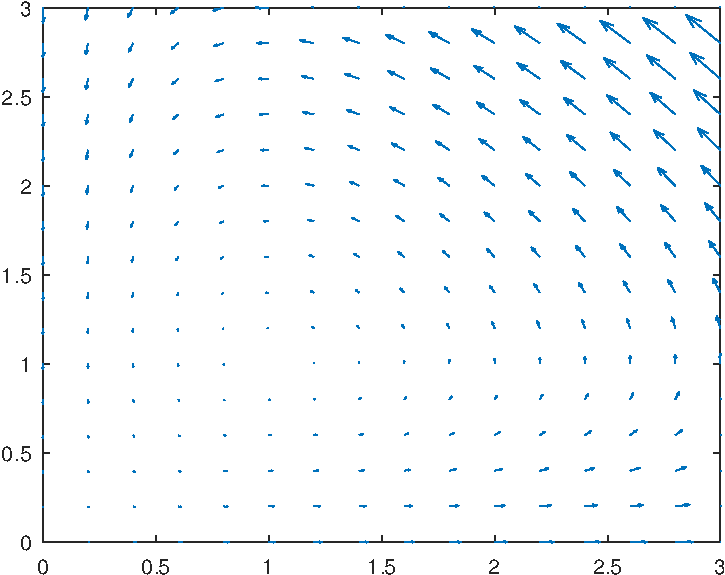
\includegraphics[width=.7\textwidth]{octave/volterra-vectors-crop.pdf}
  \end{center}
\end{frame}

\begin{frame}{Lösung im Phasenraum}
  \begin{center}
    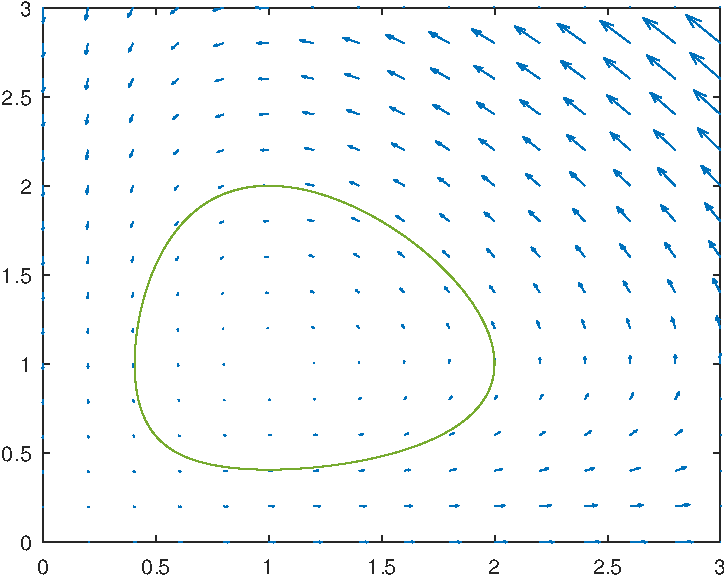
\includegraphics[width=.7\textwidth]{octave/volterra-phasespace-crop.pdf}
  \end{center}
  Eine als Beispiel berechnete Lösungskurve
\end{frame}

\begin{frame}{Lösung als Funktion der Zeit}
  \begin{center}
    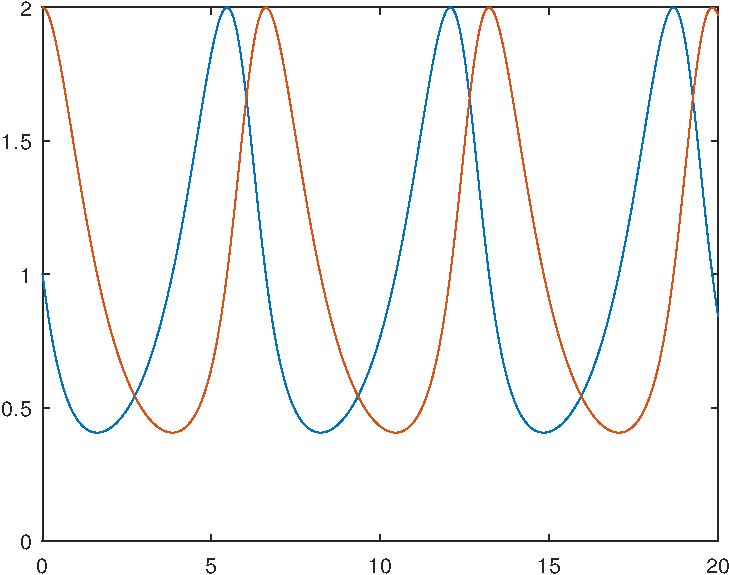
\includegraphics[width=.7\textwidth]{octave/volterra-timeseries-crop.pdf}
  \end{center}
  Die Lösung als Weg: was ist $x$, was ist $y$?
\end{frame}

\begin{frame}{Fixpunkte}
  \only<1>{
    \begin{Denkpause}
      Gibt es Fixpunkte?
    \end{Denkpause}
  }
  \pause
  \begin{itemize}
  \item Fixpunkte des Systems sind Nullstellen der rechten Seite
    \begin{gather*}
      \begin{aligned}
        x' &=& ax &-bxy\\
        y' &=& -cy & +dxy
      \end{aligned}
    \end{gather*}
  \item Offensichtlich ist $(0,0)$ ein Fixpunkt
    \begin{itemize}
    \item Es gibt keine Individuen, die sich vermehren könnten
    \end{itemize}
    \pause
  \item Ein zweiter Fixpunkt ist
    \begin{gather*}
      x=\frac cd,\qquad y=\frac ab
    \end{gather*}
    \begin{itemize}
    \item Tunfisch und Sardinen sind im Gleichgewicht
    \end{itemize}
  \end{itemize}
\end{frame}

\begin{frame}{Erhaltungssätze}
  \begin{itemize}
  \item Wir führen die folgende Größe ein:
    \begin{gather*}
      V(x,y) = dx - c \ln x + by - a \ln y
    \end{gather*}
  \item Für jede Lösung der Lotka-Volterra-Gleichungen $(x(t),y(t))$ gilt
    \begin{gather*}
      d_t V\bigl(x(t),y(t)\bigr) = 0
    \end{gather*}
    \pause
  \item Eine solche Aussage nennt man \textbf{Erhaltungssatz}, $V$
    nennt man eine \textbf{Erhaltungsgröße}
  \item Erhaltungsgrößen spielen eine wichtige Rolle für das
    Verständnis von dynamischen Systemen
  \item Mit Ihnen zeigt man Eigenschaften von Lösungen, z.B.
    \begin{itemize}
    \item beschränkt
    \item periodisch
    \end{itemize}
  \end{itemize}
  
\end{frame}

\begin{Aufgabe}
  Zeigen Sie, dass die Erhaltungsgleichung
  $d_t V\bigl(x(t),y(t)\bigr) = 0$ tatsächlich für jede Lösung der Lotka-Volterra-Gleichungen $(x(t),y(t))$ gilt.
\end{Aufgabe}

\begin{frame}
  \begin{block}{Warnung}
    Für die Lotka-Volterra-Gleichungen gibt es keine geschlossene
    Darstellung der Lösungen.
  \end{block}

  Es lassen sich aber einige Aussagen treffen
  \begin{itemize}
  \item Es gibt die beiden Fixpunkte $(0,0)^T$ und
    $\left(\tfrac cd,\tfrac ab\right)^T$
  \item Es gibt Erhaltungssätze
  \item Lösungen sind periodisch
  \end{itemize}
\end{frame}

\begin{frame}{Lösungen zu verschiedenen Anfangswerten}
  \begin{center}
    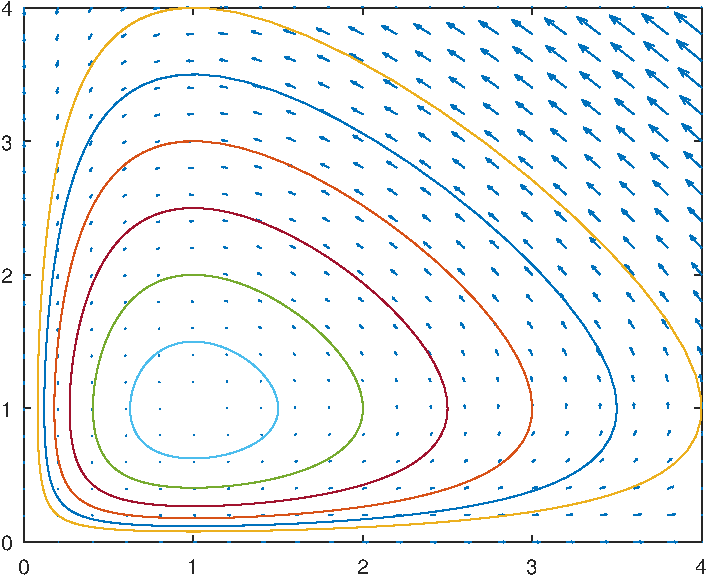
\includegraphics[width=.7\textwidth]{octave/volterra-multi-crop.pdf}
  \end{center}    
\end{frame}

\begin{frame}{Ideen zur Steuerung des Systems}
  Aufgabe: Sie wollen durch das Abfischen von Tunfisch die Sardinenpopulation erhöhen
  \begin{itemize}
  \item Wird das jederzeit funktionieren?
  \visible<3->{
    \begin{itemize}
    \item Es ist die Kenntnis der relativen Position zum Fixpunkt nötig, um gezielt zu steuern.
    \end{itemize}
  }
  \item Kann es langfristig Erfolg haben?
  \visible<4->{
    \begin{itemize}
    \item Langfristig wird das System um denselben Fixpunkt oszillieren
    \end{itemize}
  }
  \end{itemize}
  \visible<2>{
    \begin{Denkpause}
      Argumentieren Sie anhand der vorherigen Grafik
    \end{Denkpause}
  }
  \visible<5>{
    \begin{block}{}
      Wir haben soeben einen ersten Einblick in die Steuerung dynamischer Systeme gewonnen
    \end{block}
  }
\end{frame}

\begin{onlyenv}<article>
  \begin{envgkerror}{Ausarbeiten}
    \begin{Aufgabe}
      \begin{enumerate}
      \item Modifizieren Sie die Lotka-Volterra-Gleichungen für den
        Fall, dass Tunfische mit einer Rate $ey$ gefangen werden.
      \item Finden Sie Fixpunkte der modifizierten Gleichungen
      \item Skizzieren Sie das zugehörige Vektorfeld
      \end{enumerate}
    \end{Aufgabe}
  \end{envgkerror}
\end{onlyenv}

\begin{Abschluss}
\item Was wird im Phasenraumdiagramm dargestellt?
\item Welcher Bezug besteht zwischen Vektorfeld und der Kurve einer Lösung?
\item Wie erkennen Sie stationäre Punkte?
\item Wie erkennen Sie die Auswirkung von Eingriffen in das System?
\end{Abschluss}

%%%%%%%%%%%%%%%%%%%%%%%%%%%%%%%%%%%%%%%%%%%%%%%%%%%%%%%%%%%%%%%%%%%%%%
%%%%%%%%%%%%%%%%%%%%%%%%%%%%%%%%%%%%%%%%%%%%%%%%%%%%%%%%%%%%%%%%%%%%%%
\subsection{Kompartimentmodelle in der Epidemiologie}

\begin{frame}{Kompartimentmodelle}
  \begin{itemize}
  \item Komplexe Verhältnisse werden durch wenige diskrete \glqq{}Kompartimente\grqq{} (compartments) ersetzt
    \begin{itemize}
    \item Personengruppen in der Epidemiologie
    \item Regionen in Zellen
    \end{itemize}
  \item Jedes der Kompartimente wird homogen angenommen
    \begin{itemize}
    \item Bzgl. des Modell gleiche Eigenschaften
    \item Vollständige Durchmischung
    \item Epidemiologie: keine räumliche Auflösung
    \end{itemize}
  \item Der Austausch zwischen den Gruppen ist homogen
    \begin{itemize}
    \item Epidemiologie: die Wahrscheinlichkeit, jemanden aus einer
      der Gruppen zu treffen ist gleich
    \item Das zusammentreffen von Personen ist zeitlich homogen
    \end{itemize}
  \end{itemize}
\end{frame}

\begin{frame}{Das SIR-Modell}
  Drei Personengruppen mit konstanter Gesamtzahl $N$
  \begin{gather*}
    N = S+I+R
  \end{gather*}
  \begin{description}
  \item[Susceptible] $S$ Personen, die sich anstecken können
  \item[Infectious] $I$ infizierte Personen, die die Krankheit weitergeben können
  \item[Removed] $R$ Personen, die nach der Erkrankung immun sind
  \end{description}
  \pause
  \begin{block}{Ethische Komponente}
    In diesen Modellen werden Personen nicht mehr als Menschen
    betrachtet, sondern als komponenten in einem mathematischen
    System. So nützlich Modelle dieser Art sind, so sind sie doch
    prinzipiell nicht mit §1 GG verträglich. Das muss bei ihrer
    Anwendung immer berücksichtigt werden.
  \end{block}
\end{frame}

\begin{frame}{Übergänge zwischen den Gruppen}
  \begin{description}
  \item[$S\to I$] Eine Person $S$ trifft eine infektiöse Person $I$ und wird mit
    der Wahrscheinlichkeit $\hat \beta$ infiziert.
    \begin{itemize}
    \item Personen treffen kontinuierlich andere Personen mit der Rate $m$ pro Zeiteinheit
    \item Die Wahrscheinlichkeit, dass die andere Person infektiös ist, ist $I/N$.
    \end{itemize}
  \item[$I\to R$] Eine infizierte Person erholt sich oder stirbt mit
    einer Rate $\gamma$ pro Zeiteinheit
  \end{description}
  \pause Anmerkung: $\hat\beta$ ist die Übertragungswahrscheinlichkeit
  einer Begegnung. Wir machen die Annahme, dass die Übertragungsrate
  linear mit der Anzahl der Begegnunen wächst und setzen
  $\beta = m \hat\beta$. Auf diese Art sind alle Parameter bezüglich
  derselben Zeiteinheit, typischerweise Tage.
\end{frame}

\begin{frame}{Die Gleichungen}
  \begin{block}{In der Einheit \glqq{}Personen\grqq{}}

    \only<presentation>{\vspace*{-2ex}}
    \begin{align*}
      d_t S &=-\beta S\frac IN\\
      d_t I &=\beta S\frac IN - \gamma I\\
      d_t R &=\gamma I
    \end{align*}  
  \end{block}

  \begin{onlyenv}<article> Die Gleichungen in der Einheit Personen
    sind mathematisch unhandlich, auch wenn die Ergebnisse sofort
    anwendbar sind. Eleganter ist die Darstellung un
    Bevölkerungsanteilen, indem jede Größe durch $N$ dividiert
    wird. Da damit auch die Ableitung entsprechend dividiert wird,
    werden die Gleichungen unabhängig von $N$ und gelten für beliebige
    Bevölgerungen.
  \end{onlyenv}
  \begin{block}{In der Einheit \glqq{}Bevölkerungsanteil\grqq{}}
    \only<presentation>{\vspace*{-2ex}}
    \begin{align*}
      d_t S &=-\beta SI\\
      d_t I &=\beta SI - \gamma I\\
      d_t R &=\gamma I
    \end{align*}  
  \end{block}
\end{frame}

\begin{frame}{Eigenschaften der Lösung}
  \begin{align*}
    d_t S &=-\beta SI\\
    d_t I &=\beta SI - \gamma I\\
    d_t R &=\gamma I
  \end{align*}  
  \begin{itemize}
  \item Alle Größen liegen im Intervall $[0,1]$
    \begin{itemize}
    \item Folgt aus dem Ansatz als Bevölkerungsanteil
    \item Muss für Lösungen überprüft werden
    \end{itemize}
  \item $S$ ist monoton fallend und $R$ steigend
    \begin{itemize}
    \item Daher konvergieren beide für $t\to\infty$
    \end{itemize}
  \item Jeder Punkt $(S,0,R)$ ist ein Fixpunkt
  \end{itemize}
\end{frame}

\begin{frame}{Reproduktionszahlen}
  \begin{gather*}
    d_t I = \beta SI-\gamma I = (R_0S-1) \gamma I
  \end{gather*}
  \begin{block}{Basisreproduktionszahl $R_0$}
    $R_0$ gibt an, wieviele Personen von einer infektiösen Person
    angesteckt werden, wenn $S\approx 1$, also zu Beginn der
    Epidemie. Sie ergibt sich als
    \begin{gather*}
      R_0 = \frac\beta\gamma
    \end{gather*}
  \end{block}

  \begin{block}{Effektive Reproduktionszahl $R_e$}
    $R_e = SR_0$ gibt an, wieviele Personen im Verlauf der Epidemie
    von einer infektiösen Person angesteckt werden.
  \end{block}
\end{frame}

\begin{frame}
  \frametitle<presentation>{Entwicklung von $I$}
  \begin{gather*}
    d_t I = (R_e-1) \gamma I
  \end{gather*}
  \begin{description}
  \item[$R_e>1$] Die Anzahl der Infektiösen wächst
    \begin{itemize}
    \item Für $R_0>1$ beginnt die Epidemie mit exponentiellem Wachstum
    \item Dies wird gebremst, wenn $S$ deutlich unter 1 liegt
    \end{itemize}
  \item[$R_e<1$] Die Anzahl der Infektiösen schrumpft
    \begin{itemize}
    \item Für $R_0<1$ bricht keine Epidemie aus
    \item Im Endstadium schrumpft die Zahl der Infektiösen exponenziell
    \end{itemize}
  \item[$R_e=1$] Grenzfall $d_t I = 0$
    \begin{itemize}
    \item Falls $I>0$, ist $S$ streng monoton fallend, es ist also kein Fixpunkt
    \item Eintritt der \glqq{}Herdenimmunität\grqq{}
    \end{itemize}
  \end{description}
\end{frame}

\begin{frame}{Der Grenzwert für unendliche Zeit}
  \begin{itemize}
  \item Wir haben bereits gesehen:
    \begin{itemize}
    \item $I\to 0$ wenn $t\to \infty$
    \item Die Grenzwerte $S_\infty$ und $R_\infty$ existieren 
    \end{itemize}
  \item Es gilt dann $S_\infty+R_\infty = 1$
  \item Aufwändige mathematische Berechnungen ergeben
    \begin{gather*}
      S_\infty = e^{R_0(S_\infty-1)}
    \end{gather*}
    \begin{itemize}
    \item Beispiel für $R_0=3$ ist $S_\infty \approx 5.95\%$
    \end{itemize}
  \end{itemize}
\end{frame}

\begin{Aufgabe}
  \begin{enumerate}
  \item Modifizieren Sie das SIR-Modell, so dass die Immunität der Gruppe
  $R$ exponentiell abklingt.
  \item Welche Grundannahmen der Analyse für $t\to\infty$ ändern sich dadurch?
  \end{enumerate}
\end{Aufgabe}

\begin{frame}{Das SEIR-Modell}
  \begin{itemize}
  \item Modellierung von Inkubationszeiten
  \item Zusätzlich zum SIR-Modell fügen wir eine weitere Gruppe hinzu
    \begin{itemize}
    \item $E$ (exposed) Infiziert, aber (noch) nicht infektiös
    \end{itemize}
  \item Es gibt eine Übergangsrate $\sigma$ von $E$ nach $I$
  \end{itemize}
  \begin{align*}
    d_t S &=-\beta SI\\
    {\color{blue}d_t E} &{\color{blue}=\beta SI - \sigma E}\\
    d_t I &={\color{blue}\sigma E} - \gamma I\\
    d_t R &=\gamma I
  \end{align*}  
\end{frame}

\begin{frame}{Schwächen der Modelle}
  Im Plenum möchte ich gern diskutieren, wo bei den SIR- und
  SEIR-Modellen eine fundamentale Schwäche liegt und wie man sie
  beheben sollte.
\end{frame}

\begin{frame}{Was ist ein mathematisches Modell}
  \begin{itemize}
  \item Es ist ein System von mathematischen Formeln, das den
    modellierten Prozess mit einer für die Anwendung hinreichenden
    Genauigkeit beschreibt
  \item Es ist eine Abstraktion und damit Vereinfachung
  \item Es beruht auf expliziten Annahmen und erlaubt Schlüsse aus diesen
  \item Es ist in dem Sinne überprüfbar, dass Messwerte und Rechnungen
    hinreichend nah beieinander liegen
  \item Es ist \textbf{nicht} eine wahre oder falsche Aussage über die Natur
  \end{itemize}
\end{frame}

\begin{Abschluss}
\item Was ist ein Kompartimentmodell?
\item Wie modellieren Sie die \glqq{}Reaktion\grqq{} zwischen zwei Gruppen?
\item Welche Grundannahmen stecken im SIR-Modell
\item Wie entwickeln sich seine Lösungen mit der Zeit?
\end{Abschluss}

%%%%%%%%%%%%%%%%%%%%%%%%%%%%%%%%%%%%%%%%%%%%%%%%%%%%%%%%%%%%%%%%%%%%%%
%%%%%%%%%%%%%%%%%%%%%%%%%%%%%%%%%%%%%%%%%%%%%%%%%%%%%%%%%%%%%%%%%%%%%%
\subsection{Integrierende Faktoren für lineare Differentialgleichungen}

\begin{frame}{Lineare Differentialgleichungen}
  In diesem Abschnitt wollen wir eine Lösungsmethode für lineare
  Differentialgleichungen, also Gleichungen der Form
  \begin{gather*}
    x'(t) = a(t) x(t) + b(t)
  \end{gather*}
  herleiten. Für den Fall $a(t)\equiv a$ konstant und $b(t)\equiv 0$
  kennen wir bereits die Lösungen
  \begin{gather*}
    x(t) = c e^{at}.
  \end{gather*}
\end{frame}

\begin{frame}{Einführung von Differentialoperatoren}
  \begin{itemize}
  \item Zu jeder Differentialgleichung gehört ein Differentialoperator
    $L$, so dass $L[x]$ alle Terme mit der Lösung $x$ und ihren
    Ableitungen enthält.
  \item Beispiel:
    \begin{gather*}
      x'(t) = a(t) x(t) + b(t)
      \qquad\Rightarrow\qquad
      L[x](t) = x'(t) - a(t)x(t)
    \end{gather*}
  \item Die Differentialgleichung wird damit zu
    \begin{gather*}
      L[x](t) = b(t).
    \end{gather*}
  \item
    Eine solche Gleichung heißt \textbf{homogen}, wenn $b(t)\equiv 0$ gilt.
  \end{itemize}
\end{frame}

\begin{frame}{Was bedeutet linear?}
  \begin{itemize}
  \item Ein Differentialoperator $L$ und die zugehörige
    Differentialgleichung heißen \textbf{linear}, wenn für beliebige
    differenzierbare Funktionen $x$, $y$ und Zahlen $a$, $b$ gilt
    \begin{gather*}
      L[ax+by] = aL[x] + bL[y]
    \end{gather*}
  \item Ist $L$ linear, so gilt für zwei Lösungen der homogenen Differentialgleichung
    \begin{gather*}
      L[x] = 0,\qquad L[y]=0,
    \end{gather*}
    dass auch für Linearkombinationen der Lösungen gilt
    \begin{gather*}
      L[ax+by] = 0
    \end{gather*}
  \end{itemize}
\end{frame}

\begin{frame}
  \begin{block}{Notation}
    Wir werden im Folgenden Integrale als Argumente in die
    Exponentialfunktion einsetzen. Da das schwer lesbar wird, führen
    wir ein:
    \begin{gather*}
      \exp(x) = e^x
    \end{gather*}
  \end{block}

  Insbesondere ist dann
  \begin{gather*}
    \exp\left(\int_{t_0}^t a(s)\,ds\right) =
    e^{\int_{t_0}^t a(s)\,ds}
  \end{gather*}
\end{frame}

\begin{frame}{Integrierende Faktoren}
\end{frame}

%%%%%%%%%%%%%%%%%%%%%%%%%%%%%%%%%%%%%%%%%%%%%%%%%%%%%%%%%%%%%%%%%%%%%%
%%%%%%%%%%%%%%%%%%%%%%%%%%%%%%%%%%%%%%%%%%%%%%%%%%%%%%%%%%%%%%%%%%%%%%
\subsection{Lösung linearer Systeme von Dgln.}

\begin{frame}
  \begin{block}{Lineares System von Differentialgleichungen}
    Ein lineares System von DGl. erster Ordnung der Dimension $n$ hat
    die Form
    \begin{gather*}
      x' = Ax + f
      \qquad\text{oder}\qquad
      x'(t) = A(t)x(t) + b(t)
    \end{gather*}
    Es sind $x(t), x'(t), b(t) \in \R^n$ und $A(t)\in \Rnn$.
    
    Falls $A$ und $b$ nicht von der Zeit $t$ abhängen, ist das System
    autonom, es ist homogen, falls $b\equiv0$.
  \end{block}

  \begin{block}{Lösung der AWA im homogenen, autonomen Fall}
    Wie im Falle der linearen Wachstumsgleichung schreiben wir die
    Lösung der Anfangswertaufgabe mit einem Startvektor $x(0) = x_0\in\R^n$:
    \begin{gather*}
      x(t) = e^{At} x_0.
    \end{gather*}
  \end{block}
\end{frame}

\begin{frame}{Exponentialfunktion einer Diagonalmatrix}
\end{frame}

\begin{frame}{Exponentialfunktion einer diagonalisierbaren Matrix}
  
\end{frame}

\begin{frame}{Eigenschaften der Matrix-Exponentialfunktion}
  Für beliebige Matrizen $A$ und invertierbare Matrizen $S$ gilt
  \begin{align*}
    e^0 &= \mathbb I\\
    e^{S^{-1}AS} &= S^{-1} e^A S\\
    e^{\alpha A} e^{\beta A} &= e^{(\alpha+\beta) A}\\
    e^{A}e^{-A} &= \mathbb I\\
  \end{align*}
  \begin{itemize}
  \item Aus der letzten Gleichung folgt insbesondere, dass $e^A$ für jede
    Matrix $A$ invertierbar ist und $e^{-A}$ die Inverse ist.
  \item Aus der zweiten Eigenschaft folgt, dass die Eigenvektoren von
    $e^A$ identisch mit denen von $A$ sind.
  \end{itemize}
\end{frame}

\begin{frame}{Beispiel}
  \begin{gather*}
    A =
    \begin{pmatrix}
      0 & 1\\k^2 & 0
    \end{pmatrix},
    \qquad \lambda_{1/2} = \pm k,
    \qquad v_1 =
    \begin{pmatrix}
      1\\k
    \end{pmatrix},
    \quad
    v_2 =
    \begin{pmatrix}
      1 \\ -k
    \end{pmatrix}.
  \end{gather*}
  \pause
  Sei $S$ die Matrix mit Spalten $v_1$ und $v_2$, dann gilt
  \begin{gather*}
    A = S^{-1}
    \begin{pmatrix}
      k \\ &-k
    \end{pmatrix}
    S,
    \qquad
    S^{-1} =
    \frac12
    \begin{pmatrix}
      1 & \tfrac1k\\
      1 & -\tfrac1k\\
    \end{pmatrix}
  \end{gather*}
  \pause
  Nun exponenzieren wir die Eigenwerte und erhalten
  \begin{gather*}
    e^A =  S^{-1}
    \begin{pmatrix}
      e^k \\ &e^{-k}
    \end{pmatrix}
    S
    = \frac12
    \begin{pmatrix}
      e^k + e^{-k} & \tfrac 1k (e^k - e^{-k}) \\
      k (e^k - e^{-k}) & e^k + e^{-k}
    \end{pmatrix}
    =
    \begin{pmatrix}
      \cosh(k) & \tfrac 1k \sinh(k) \\
      k \sinh(k) & \cosh(k)
    \end{pmatrix}
  \end{gather*}
  \vspace*{.9\textheight}
\end{frame}

\begin{frame}{Lösung des allgemeinen linearen Systems}
  \begin{block}{Integrierender Faktor}
    Zum System
    \begin{gather*}
      x'(t) = A(t) x(t) + b(t)
    \end{gather*}
    definieren wir den integrierenden Faktor
    \begin{gather*}
      M(t) = \exp\left(-\int_0^t A(s) \,ds\right).
    \end{gather*}
  \end{block}
  Wir beobachten, dass
  \begin{align*}
    M(0) &= \mathbb I,\\
    M'(t) &= -M(t) A(t).
  \end{align*}
\end{frame}

\begin{frame}
  \begin{block}{Lösung mit integrierendem Faktor}
    Für die Anwangswertaufgabe
    \begin{gather*}
      x'(t) = A(t)x(t)+ b(t),
      \qquad
      x(0) = x_0,
    \end{gather*}
    lässt sich die Lösung mit dem integrierenden Faktor $M(t)$ über die Formel
    \begin{gather*}
      x(t) = M^{-1}(t)
      \left(
        x_0 + \int_0^t M(s) b(s) \,ds
      \right)
    \end{gather*}
    darstellen.
  \end{block}
\end{frame}

\begin{frame}
  \begin{block}{Lösungsraum}
    Die Lösungen des homogenen, linearen Systems der Dimension $n$
    \begin{gather*}
      x'(t) = A(t)x(t)
    \end{gather*}
    bilden einen Vektorraum der Dimension $n$
  \end{block}
  \pause
  Begründung:
  \begin{enumerate}
  \item Mit zwei Lösungsfunktionen $x_1$ und $x_2$ ist auch
    $ax_1+bx_2$ eine Lösung
  \item Aufgrund der Invertierbarkeit der Exponentialfunktion bildet
    \begin{gather*}
      x_1 = M^{-1} e_1, x_2 = M^{-1} e_2,\dots, x_n = M^{-1} e_n,
    \end{gather*}
    mit der Einheitsbasis $e_1,\dots,e_n$ eine Basis.
  \end{enumerate}
\end{frame}

\begin{frame}{Fixpunkte}
  \begin{gather*}
    x' = Ax+f
  \end{gather*}
  \begin{exampleblock}{Frage}
    Welche Bedingung stellen Sie an einen Fixpunkt des Systems?
  \end{exampleblock}
\end{frame}


\begin{frame}{Fixpunkte}
  \begin{block}{Satz}
  Das autonome System
  \begin{gather*}
    x' = Ax+f
  \end{gather*}
  hat unter der Bedingung, dass $A$ invertierbar ist, genau einen Fixpunkt
  \begin{gather*}
    x_F = -A^{-1}f.
  \end{gather*}
  Das Spektrum von $A$ entscheidet dabei über den Charakter des Fixpunkts.    
  \end{block}
\end{frame}


\begin{frame}{Beispiele}
  \begin{center}
    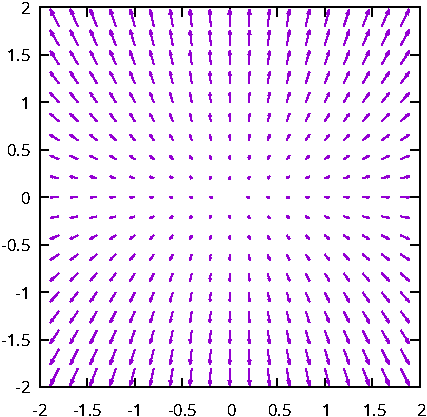
\includegraphics[width=.32\textwidth]{gnuplot/linear-pp-crop.pdf}
    \hfill
    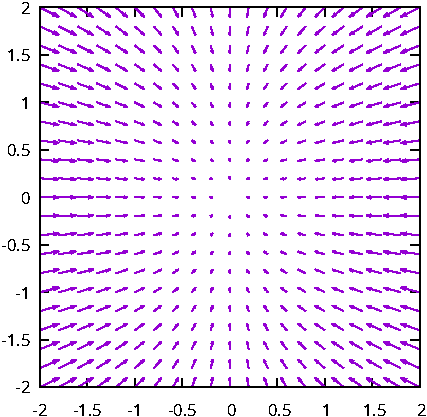
\includegraphics[width=.32\textwidth]{gnuplot/linear-mm-crop.pdf}
    \hfill
    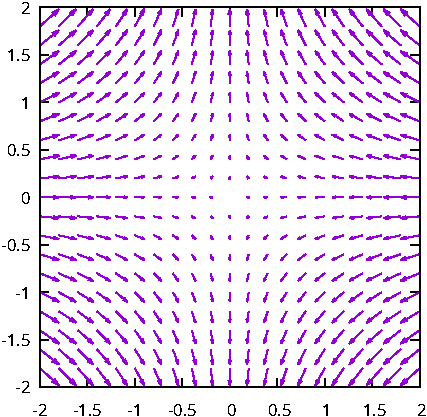
\includegraphics[width=.32\textwidth]{gnuplot/linear-pm-crop.pdf}
  \end{center}
\end{frame}

\begin{frame}
  \begin{exampleblock}{Diskussion}
    Reelle Matrizen können komplexe Eigenwerte haben. Offensichtlich
    wollen wir aber keine komplexwertigen Lösungen unserer AWA.
  \end{exampleblock}
\end{frame}

\begin{frame}{Komplexe Eigenwerte}
  \begin{block}{Satz}
    Hat eine reelle Matrix komplexe Eigenwerte, so treten sie als
    komplex konjugierte Paare mit ebensolchen Paaren von Eigenvektoren
    auf.
  \end{block}
  \pause
  Sei nun $r\pm i\phi$ ein solches Paar mit den Eigenvektoren $u\pm iv$
  \begin{align*}
    A (u\pm iv) &= {r+i\phi} (u\pm iv),\\
    e^A (u\pm iv) &= e^{r+i\phi} (u\pm iv) = e^r (\cos\phi \pm i \sin\phi)(u\pm iv).
  \end{align*}

  \vspace*{4cm}
\end{frame}

\begin{frame}
  \begin{block}{Reelle Lösungen}
    Hat die Matrix $A$ ein komplexes Eigenwertpaar
    $\lambda_{1/2} = r\pm i\phi$ mit zugehörigen Eigenvektoren
    $u\pm iv$, so ersetzen wir in der Transformationsmatrix die
    Eigenvektoren durch $u$ und $v$ und erhalten für $e^A$ eine
    quasi-Diagonalmatrix mit Block
    \begin{gather*}
      e^r
      \begin{pmatrix}
        \cos\phi & \sin\phi\\
        -\sin\phi & \cos \phi
      \end{pmatrix}
    \end{gather*}
  \end{block}
\end{frame}

\begin{frame}{Beispiele}
  \begin{center}
    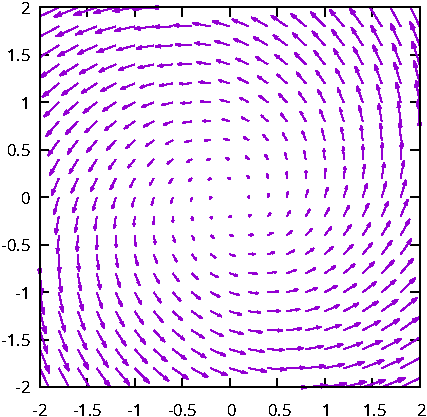
\includegraphics[width=.32\textwidth]{gnuplot/linear-cp-crop.pdf}
    \hfill
    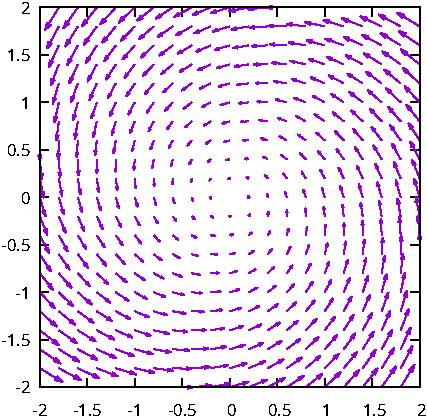
\includegraphics[width=.32\textwidth]{gnuplot/linear-cm-crop.pdf}
    \hfill
    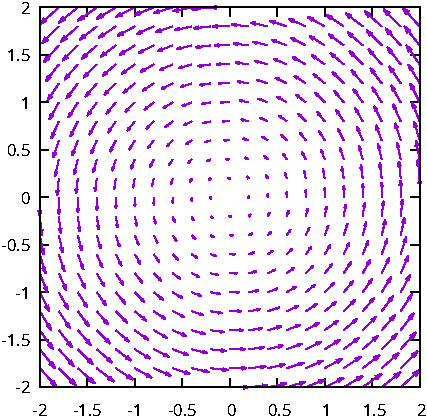
\includegraphics[width=.32\textwidth]{gnuplot/linear-c0-crop.pdf}
  \end{center}  
\end{frame}

%%%%%%%%%%%%%%%%%%%%%%%%%%%%%%%%%%%%%%%%%%%%%%%%%%%%%%%%%%%%%%%%%%%%%%
%%%%%%%%%%%%%%%%%%%%%%%%%%%%%%%%%%%%%%%%%%%%%%%%%%%%%%%%%%%%%%%%%%%%%%
\subsection{Berechnung von Lösungen anderer Gleichungen}

%%%%%%%%%%%%%%%%%%%%%%%%%%%%%%%%%%%%%%%%%%%%%%%%%%%%%%%%%%%%%%%%%%%%%%
%%%%%%%%%%%%%%%%%%%%%%%%%%%%%%%%%%%%%%%%%%%%%%%%%%%%%%%%%%%%%%%%%%%%%%
\subsection{Numerische Verfahren}



%%%%%%%%%%%%%%%%%%%%%%%%%%%%%%%%%%%%%%%%%%%%%%%%%%%%%%%%%%%%%%%%%%%%%%
%%%%%%%%%%%%%%%%%%%%%%%%%%%%%%%%%%%%%%%%%%%%%%%%%%%%%%%%%%%%%%%%%%%%%%
\begin{Abschluss}
\item Unter Annahme der Kontinuumshypothese können wir
  Wachtumsprozesse durch Differentialgleichungen
  beschreiben.
\item Populationsdynamik mehrerer Spezies führt zu Systemen von DGln.
\item Diese DGLn. haben unendlich viele Lösungen, was uns eigentlich interessiert, ist die Lösung einer Anfangswertaufgabe (AWA)
\item Das Ergebnis der eigentlichen Modellierung war die
  Volterrasche Integralgleichung
\end{Abschluss}


\begin{frame}{Zusammenfassung Analyse}
  \begin{enumerate}
  \item Qualitative Diskussion zum Verständnis der Modelle
    \begin{itemize}
    \item Richtungsfelder
    \item Phasenraumdiagramme
    \end{itemize}
  \item Verhalten für große Zeiten
    \begin{itemize}
    \item Fixpunkte
    \end{itemize}
  \item Wir haben die allgemeine Lösung der DGl. geraten und an den
    Anfangswert angeglichen
  \end{enumerate}
\end{frame}



%%%%%%%%%%%%%%%%%%%%%%%%%%%%%%%%%%%%%%%%%%%%%%%%%%%%%%%%%%%%%%%%%%%%%%
%%%%%%%%%%%%%%%%%%%%%%%%%%%%%%%%%%%%%%%%%%%%%%%%%%%%%%%%%%%%%%%%%%%%%%
%%%%%%%%%%%%%%%%%%%%%%%%%%%%%%%%%%%%%%%%%%%%%%%%%%%%%%%%%%%%%%%%%%%%%%
%%%%%%%%%%%%%%%%%%%%%%%%%%%%%%%%%%%%%%%%%%%%%%%%%%%%%%%%%%%%%%%%%%%%%%
%%%%%%%%%%%%%%%%%%%%%%%%%%%%%%%%%%%%%%%%%%%%%%%%%%%%%%%%%%%%%%%%%%%%%%


\begin{frame}
  \begin{block}{Homogene Differentialgleichungen}
    Eine Differentialgleichung ist homogen, wenn es keinen Summanden
    gibt, der die Lösungsfunktion nicht enthält. Einen solchen
    Summanden nennt man dann die Inhomogenität.
  \end{block}
  \begin{columns}
    \begin{column}[t]{.49\textwidth}
      \begin{block}{Homogen}
        \begin{gather*}
          x'+ \sin(t) x = 0
        \end{gather*}
      \end{block}
    \end{column}
    \begin{column}[t]{.49\textwidth}
      \begin{block}{Nicht homogen}
        \begin{gather*}
          x'+ \sin(t) x = 5
        \end{gather*}
      \end{block}
    \end{column}
  \end{columns}
  \only<1>{
  \begin{Denkpause}
    Welche Prozesse führen zu homogenen DGln., welche zu nicht homogenen?
  \end{Denkpause}}
\begin{itemize}
\item Homogene Gleichungen haben keine externen Quellen
\item Die null ist Lösung einer homogenen Gleichung
\end{itemize}
\end{frame}
